\label{prototype}
A prototype for solving the double sided matching problem was developed in NetLogo\footnote{Available at \url{https://ccl.northwestern.edu/netlogo/}, accessed April 28, 2016}.
In this chapter the prototype is evaluated on a discotheque example. 
In this case, it is assumed that an equal number of men and women are in a discotheque and the objective is to form couples based on the individual preferences.
Afterwards the prototype will be evaluated on more complex problems (e.g., matching students and universities and matching labour supply and labour demand).
In the following, the data model, the data generation script, the graphical user interface (GUI) and code from NetLogo will be described.

\subsection{Data Model}
According to the problem description we defined a generic data model for every individual.
This data model is valid for the discotheque example, the university and labour market example, and contains the following attributes:
\begin{itemize}
	\item id: unique object identifier
	\item name: object name (e.g. male1 or female1)
	\item maxMatchesInt: integer value representing the maximum number of matchings for this individual (e.g. in the disco example each person is maximally matched with one other person)
	\item sideInt: integer helper variable assigning an individual to one of the two participant groups
	\item partnerList: list of identifiers of the partners, ordered according to the preference of an individual
	\item rankList: list of ranks (values between 1 to 0) for the partners from the partnerList; the list is ordered from highest to lowest preferences.
	If the value is equal to 1 this partner is a perfect match.
	\item hasProposedToList: list of identifiers representing the individuals to which an individual has proposed
	\item gotProposedByList: list of identifiers representing the individuals from which an individual received proposals.
	The gotProposedByList is only valid for one iteration.
	\item tmpMatchList: list containing the identifiers of individuals to whom a temporary match was established
	\item activeFlag: boolean value stating if an individual is matched or not respectively if the individual gave up (they already proposed to all individuals from the partnerList but only received rejections)
\end{itemize}

\clearpage
\subsection{Data Generation}
In order to generate random data, which represents the individuals and their preferences the statistical computing language R\footnote{Available at \url{https://www.r-project.org/}, accessed April 28, 2016} has been used. 
The generated data is exported as a CSV list, which is then read from NetLogo. 
The R script accepts the following parameters:
\begin{itemize}
	\item seed: integer value, which is used as a seed by the number generator. The default value is 123.
	\item numberOfMen: integer value representing the number of men which should be created. The default value is 10.
	\item numberOfWomen: integer value representing the number of women which should be generated. The default value is 10.
	\item pickyLower: float value between 0 and 1 representing the lower bound which will be used in order to generate a number that represents how picky a person is. The value 0 means accepts every possible match, the value 1 excepts none.
	\item pickyUpper: float value between 0 and 1 representing the upper bound which will be used in order to generate a number that represents how picky a person is. The value 0 means excepts every possible match, the value 1 excepts none.
\end{itemize}

The script can be called as follows from the command line: 
\begin{verbatim}
Rscript initDisco.R 123 10 10 0 0
\end{verbatim}

The script generates a CSV which looks as follows:
\begin{lstlisting}[numbers=left, breaklines=true] 
"";"id";"name";"maxMatchesInt";"sideInt";"partnerList";"rankList"
"1";1;"male1";1;1;"13#18#14#17#16#11#20#19#12#15"; "0.96#0.95#0.9#0.68#0.57#0.45#0.33#0.25#0.1#0.04"
...
"11";11;"female1";1;2;"3#9#5#4#10#8#2#1#6#7"; "0.92#0.82#0.7#0.67#0.48#0.41#0.35#0.25#0.22#0.05"
\end{lstlisting}

\clearpage
\subsection{GUI}
One of the main goals in the design phase was to keep the GUI simple and clear.
The GUI was structured in two main parts - the control and the information section.
\begin{figure}[H]	
  \centering
  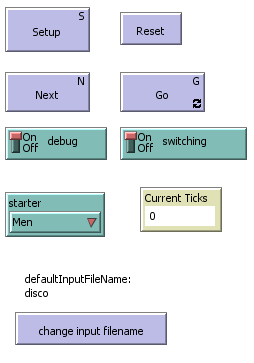
\includegraphics[width=0.5\textwidth]{netlogo-controls}
	\caption{The control section for the disco example}
	\label{fig:control-disco-gui}
\end{figure}
Figure~\ref{fig:control-disco-gui} shows the control section in the GUI. 
With the buttons \textbf{Setup} and \textbf{Reset} the simulation model can be initialized or reset after a simulation run.
The button \textbf{Next} advises the program to perform one simulation step, if \textbf{Go} is activated the simulation continues until a termination criterion is met.
In the disco example the main termination criterion is if every proposing person is already matched to another person. 
Another criterion for termination is if the proposing person already proposed to every person in his partnerList but got rejected every time.
The \textbf{debug} switch enables or disables debug messages which are printed during the setup phase and simulation run.
The speed of a simulation run can be increased if the \textbf{debug} switch is set to Off.
The second switch, \textbf{switching}, controls, if the two parties propose to each other alternatively (On) or if only one party proposes to the other one (Off).
With the drop-down list \textbf{starter} the user can determine which party starts proposing.
The reporting box \textbf{Current Ticks} shows the current number of simulation steps.
The button change input file name raises a dialogue box where the user can enter the filename of an input file which shall be used in the simulation.
Together with the number of ticks the file name will also be used as the name for the CSV export file.
\begin{figure}[H]
  \centering
  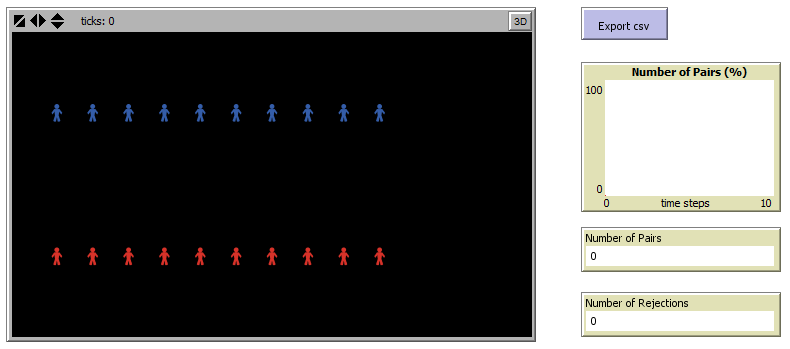
\includegraphics[width=1\textwidth]{netlogo-information}
	\caption{The information section for the disco example}
	\label{fig:info-disco-gui}
\end{figure}
Figure~\ref{fig:info-disco-gui} shows the information section of the disco example GUI. 
All created humans are shown in the world area. 
Men are coloured blue and women are red.
On setup of the simulation the proposing site is shown in the top row. 
As soon as two people are matched their colour changes to green and a link between the two is established.
If a couple is divorced the link is removed and the colour changes back to the original one.
The plot named \textbf{Number of Pairs (\%)} illustrates at each point in time how many of the possible couples exist. 
If the simulation contains 10 men and 10 women and currently 4 couples exist, the plot shows that 40\% are matched.
The reporting box \textbf{Number of Pairs} shows the absolute number of couples.
The other reporting box, \textbf{Number of Rejections}, indicates how many couples were divorced over time.
With the button \textbf{Export CSV} the current properties of all humans are exported to a CSV file.
The file name is a combination of the input file name, the starting side, if the switching is activated and the current number of ticks.

\clearpage
\subsection{NetLogo Code}
At the beginning of the NetLogo code the extensions, the data model and the needed global variables are defined.
The rest of the code is based on procedures (i.e. a sequence of NetLogo commands which begins with \textit{to} and ends with \textit{end}).
The most important procedures are the following:
\begin{itemize}
	\item \textit{setup} and \textit{reset}: both clear all results and reset the whole model to an initial empty state. 
	\item \textit{open-file}: procedure used to open a CSV list which represents the individuals and their preferences. 
	\item \textit{setup-globals}: procedure used to set up all global variables (e.g., current number of pairs, shape of the humans, etc.)
	\item \textit{step}: procedure which represents going one step in the double sided matching algorithm. The proposing site proposes and the proposals are also processed.
	\item \textit{go}: calls step until a termination criterion is met.
	\item \textit{calc-stats}: calculate some statistical information (e.g., number of pairs, number of rejections).
	\item \textit{clear-before-match}: empties the list of the proposals as a preparation for the next matching round.
	\item \textit{propose-to[sender receiver]}: sends the proposals.
	\item \textit{process-proposals [tmpId]}: processes the proposals.
	\item \textit{reject-proposals [tmpId rejectList]}: rejects the proposals.
	\item \textit{create-tmpCouples [tmpId acceptList]}: creates temporary couples.
\end{itemize}

\clearpage
\subsection{Simulation Runs}
The discotheque problem was simulated three times: once with a simple and small dataset of 20 persons (10 men and 10 women) and twice with a dataset of 200 persons (100 men and 100 women).

\subsubsection{Simulation Run 1: Small Dataset}
In the first simulation a dataset which represents 20 individuals (10 males and 10 females) was used. 
This dataset was generated using the previously described R script.
After the first simulation step there were already 6 couples (see figure \ref{fig:sim1_step1}).
\begin{figure}[H]
  \centering
  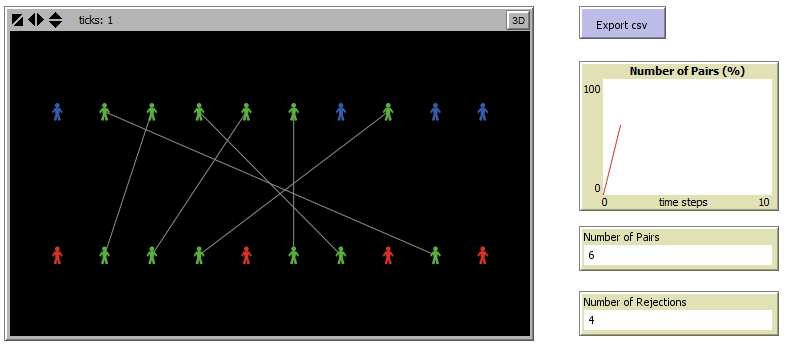
\includegraphics[width=1\textwidth]{sim1_step1}
	\caption{Simulation 1, step 1}
	\label{fig:sim1_step1}
\end{figure}

In the next few steps the number of couples continued to increase by 1 at each step. 
After the third step 8 couples were formed (see figure \ref{fig:sim1_step3}).
\begin{figure}[H]
  \centering
  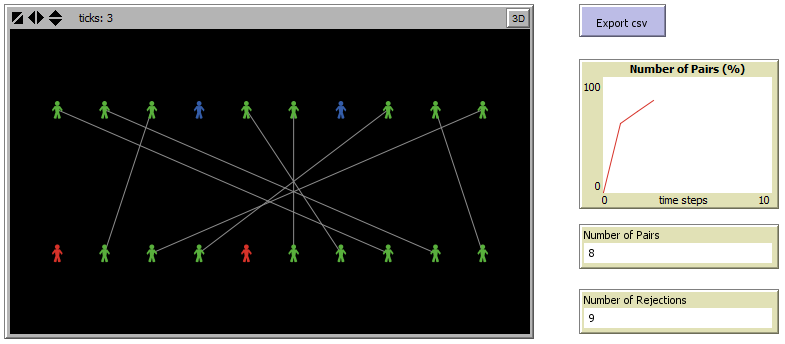
\includegraphics[width=1\textwidth]{sim1_step3}
	\caption{Simulation 1, step 3}
	\label{fig:sim1_step3}
\end{figure}

Afterwards the number of couples continued to increase slowly and some of them changed according to the individuals preferences. 
As we can see in the figure \ref{fig:sim1_step9} the male number 10 (upper right corner) was in a couple with female number 3, however male number 10 is now single, because female number 3 is now in a couple with male number 6 which is better according to their preferences.
\begin{figure}[H]
  \centering
  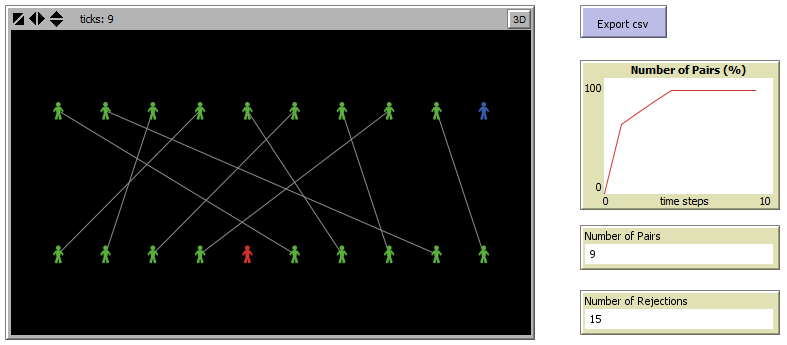
\includegraphics[width=0.8\textwidth]{sim1_step9}
	\caption{Simulation 1, step 9}
	\label{fig:sim1_step9}
\end{figure}

In the further steps, the couples continued to change according to the individuals preferences and finally after 27 steps the double sided matching problem was solved and 10 couples have been created (see figure \ref{fig:sim1_step27}).
\begin{figure}[H]
  \centering
  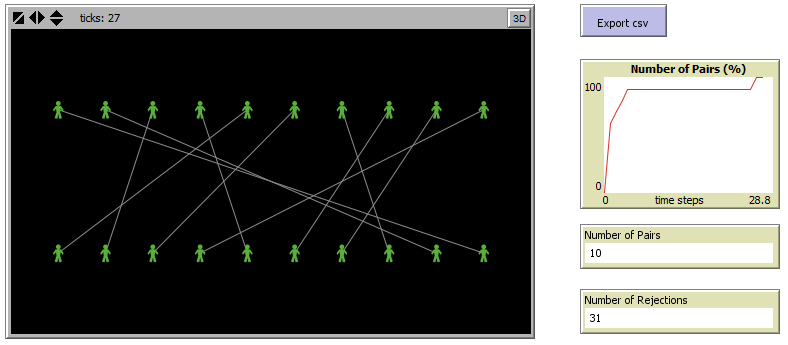
\includegraphics[width=1\textwidth]{sim1_step27}
	\caption{Simulation 1, step 27}
	\label{fig:sim1_step27}
\end{figure}

\clearpage
\subsubsection{Simulation Run 2: Large Dataset}
The second simulation consisted of a dataset representing 100 men and 100 women. 
In the first step of the simulation 49 couples were formed (see figure \ref{fig:sim2_step1}).
\begin{figure}[H]
  \centering
  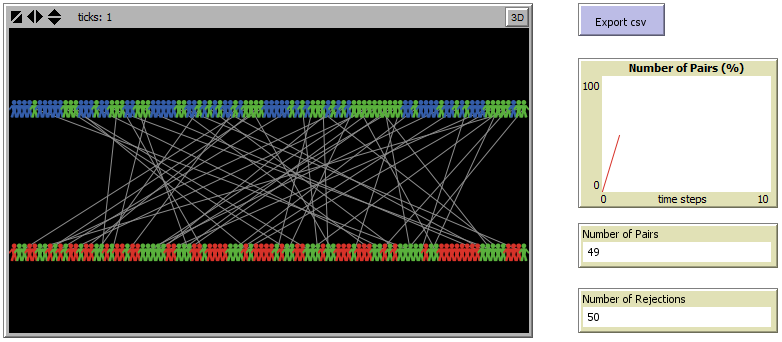
\includegraphics[width=1\textwidth]{sim2_step1}
	\caption{Simulation 2, step 1}
	\label{fig:sim2_step1}
\end{figure}

As observed in the previous simulation, in the next few steps the number of formed couples continued to increase (see figure \ref{fig:sim2_step3}).
\begin{figure}[H]
  \centering
  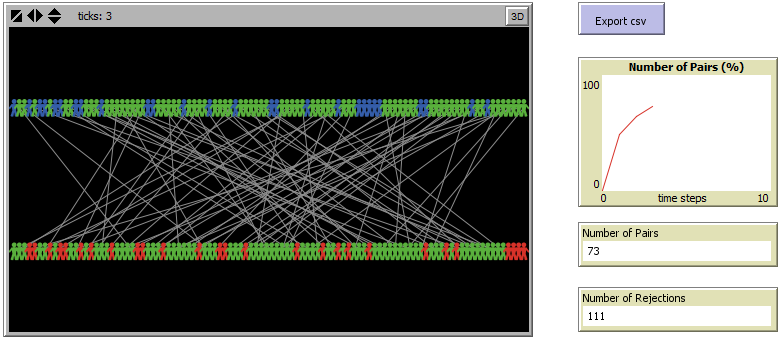
\includegraphics[width=1\textwidth]{sim2_step3}
	\caption{Simulation 2, step 3}
	\label{fig:sim2_step3}
\end{figure}

As the number of steps continued to increase the number of couples increased slowly and a change in the partners was observed (see figure \ref{fig:sim2_step9}).
\begin{figure}[H]
  \centering
  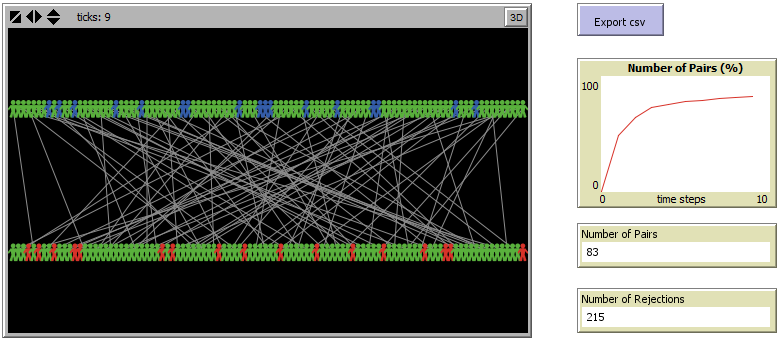
\includegraphics[width=1\textwidth]{sim2_step9}
	\caption{Simulation 2, step 9}
	\label{fig:sim2_step9}
\end{figure}

As the simulation went on, the model started to reach a stable point, where the couples increased only slowly and the number of rejections increased much faster. 
Finally after 127 steps the model has reached a final state where 94 couples were formed.
The final state of the model is illustrated in figure \ref{fig:sim2_step127}.
\begin{figure}[H]
  \centering
  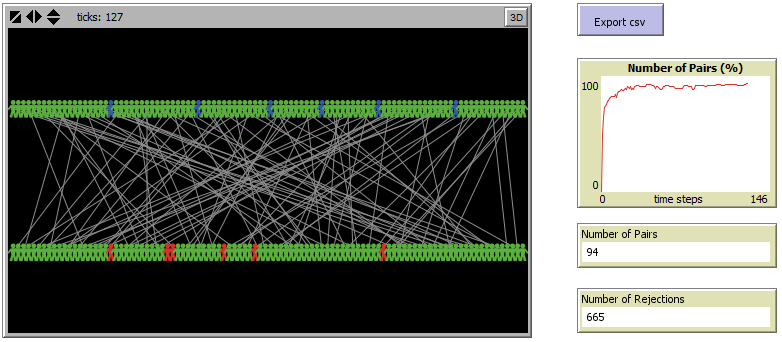
\includegraphics[width=1\textwidth]{sim2_step127}
	\caption{Simulation 2, step 127}
	\label{fig:sim2_step127}
\end{figure}

\clearpage
\subsubsection{Simulation Run 3: Large Dataset and Lower Preferences}
The second simulation was repeated with a similar dataset, but where the individuals did not have too many preferences (i.e., they were not so picky) regarding their partner.
During this simulation the couples were formed faster. After the first step (see figure \ref{fig:sim3_step1_not_picky}) there were 59 couples formed (compared to 49 from the previous simulation - see figure \ref{fig:sim2_step1}).
\begin{figure}[H]
  \centering
  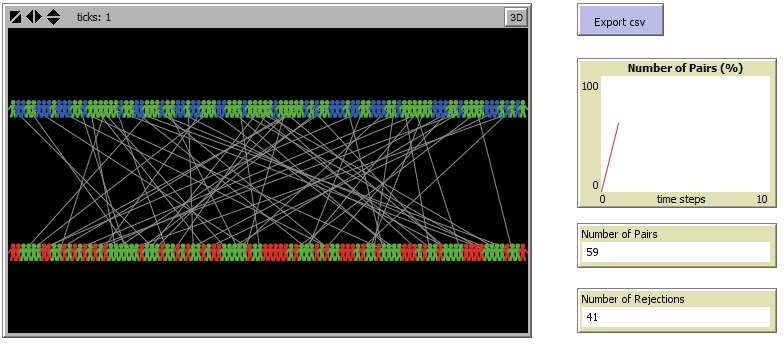
\includegraphics[width=1\textwidth]{sim3_step1_not_picky}
	\caption{Simulation 3, step 1}
	\label{fig:sim3_step1_not_picky}
\end{figure}

After the third step there were 79 (compared to 73 from the previous simulation) and after the ninth step there were 90 (compared to 83) couples.
Finally the model reached a stable state after 118 steps, where 100 couples were formed.
Another observation that was made with the new dataset is that the number of rejections was much lower than in the previous simulation. 
In the end there were 465 rejections (see figure \ref{fig:sim3_step118_not_picky}) compared to 665 from the previous run (see figure \ref{fig:sim2_step127}).
\begin{figure}[H]
  \centering
  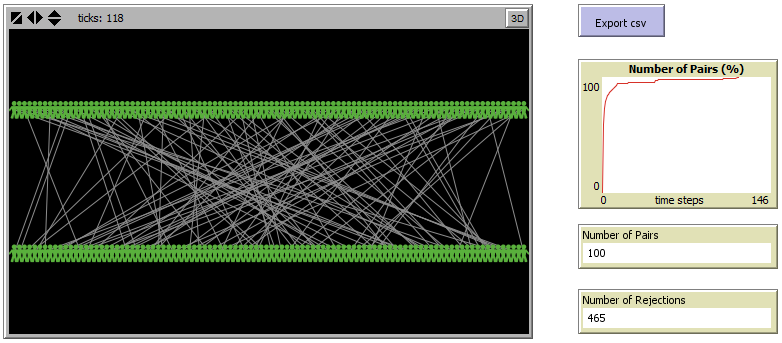
\includegraphics[width=1\textwidth]{sim3_step118_not_picky}
	\caption{Simulation 3, step 118}
	\label{fig:sim3_step118_not_picky}
\end{figure}
